\chapter{Schema di collegamento}
\section{Sketch Arduino - lato client}
\begin{figure}[!ht]
	\centering
	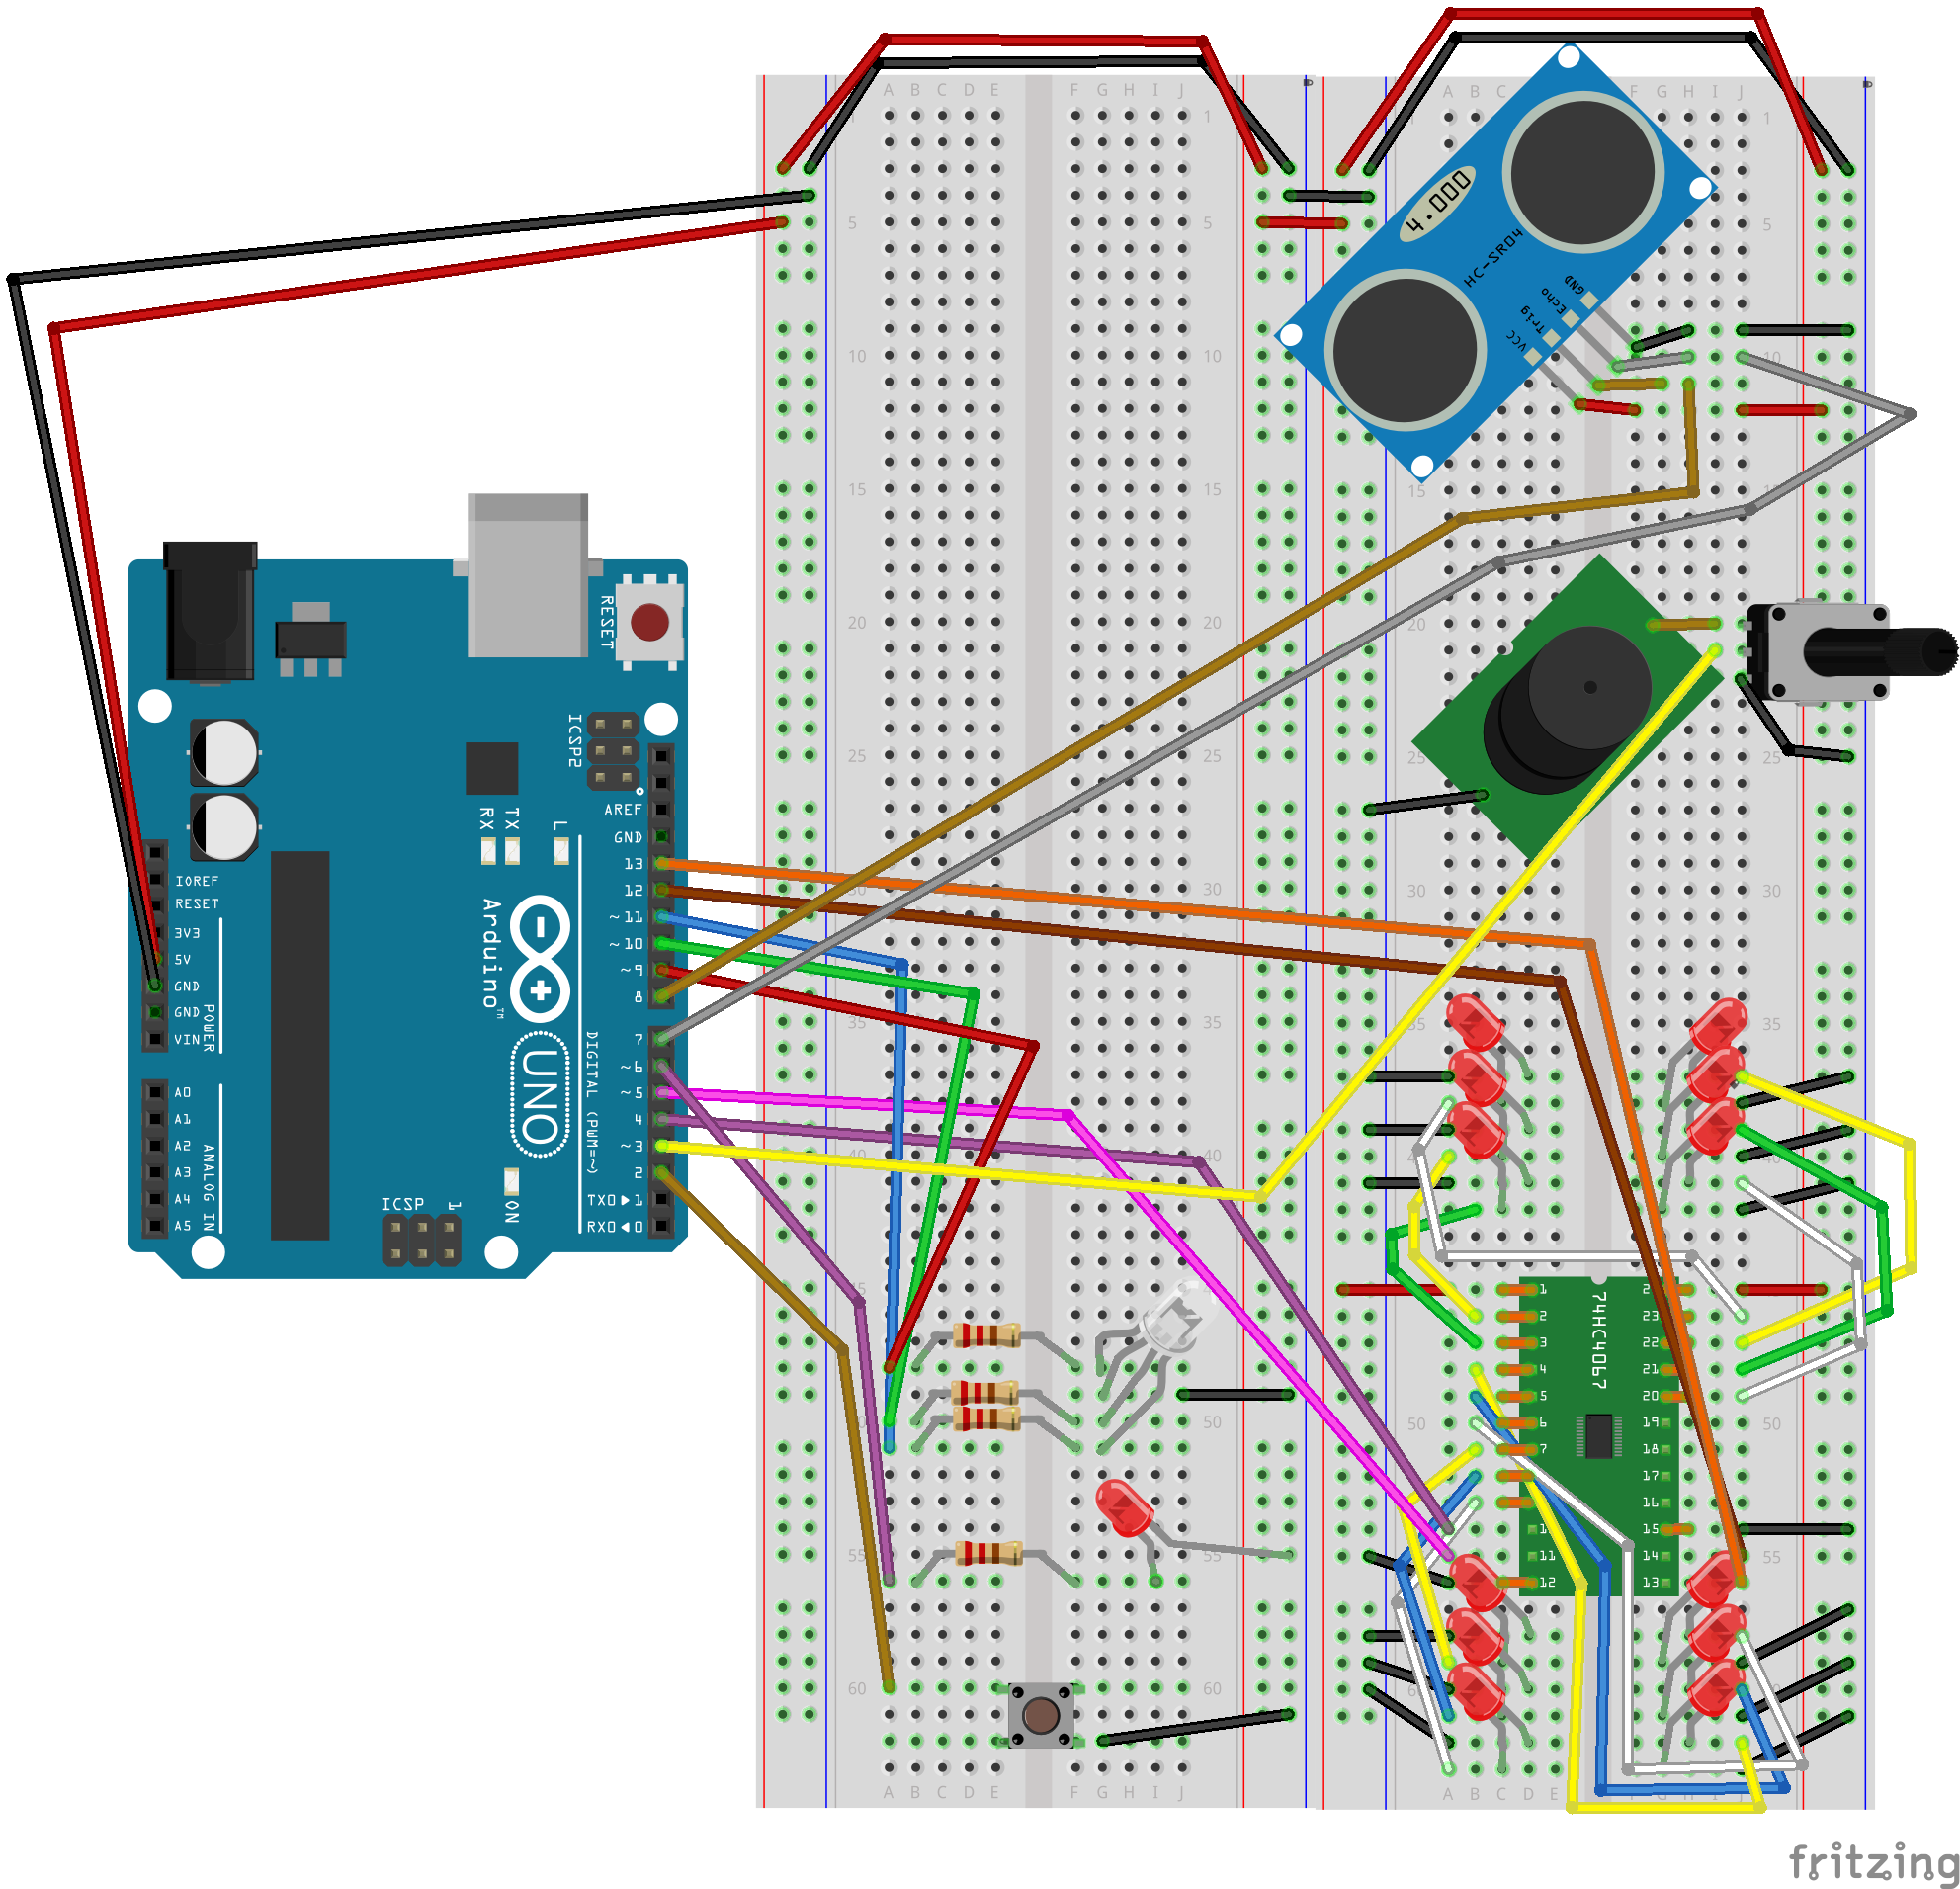
\includegraphics[scale=.60]{img/SketchClient_img.png}
	\caption{Sketch Arduino - lato client}
\end{figure}

\begin{figure}[!ht]
	\centering
	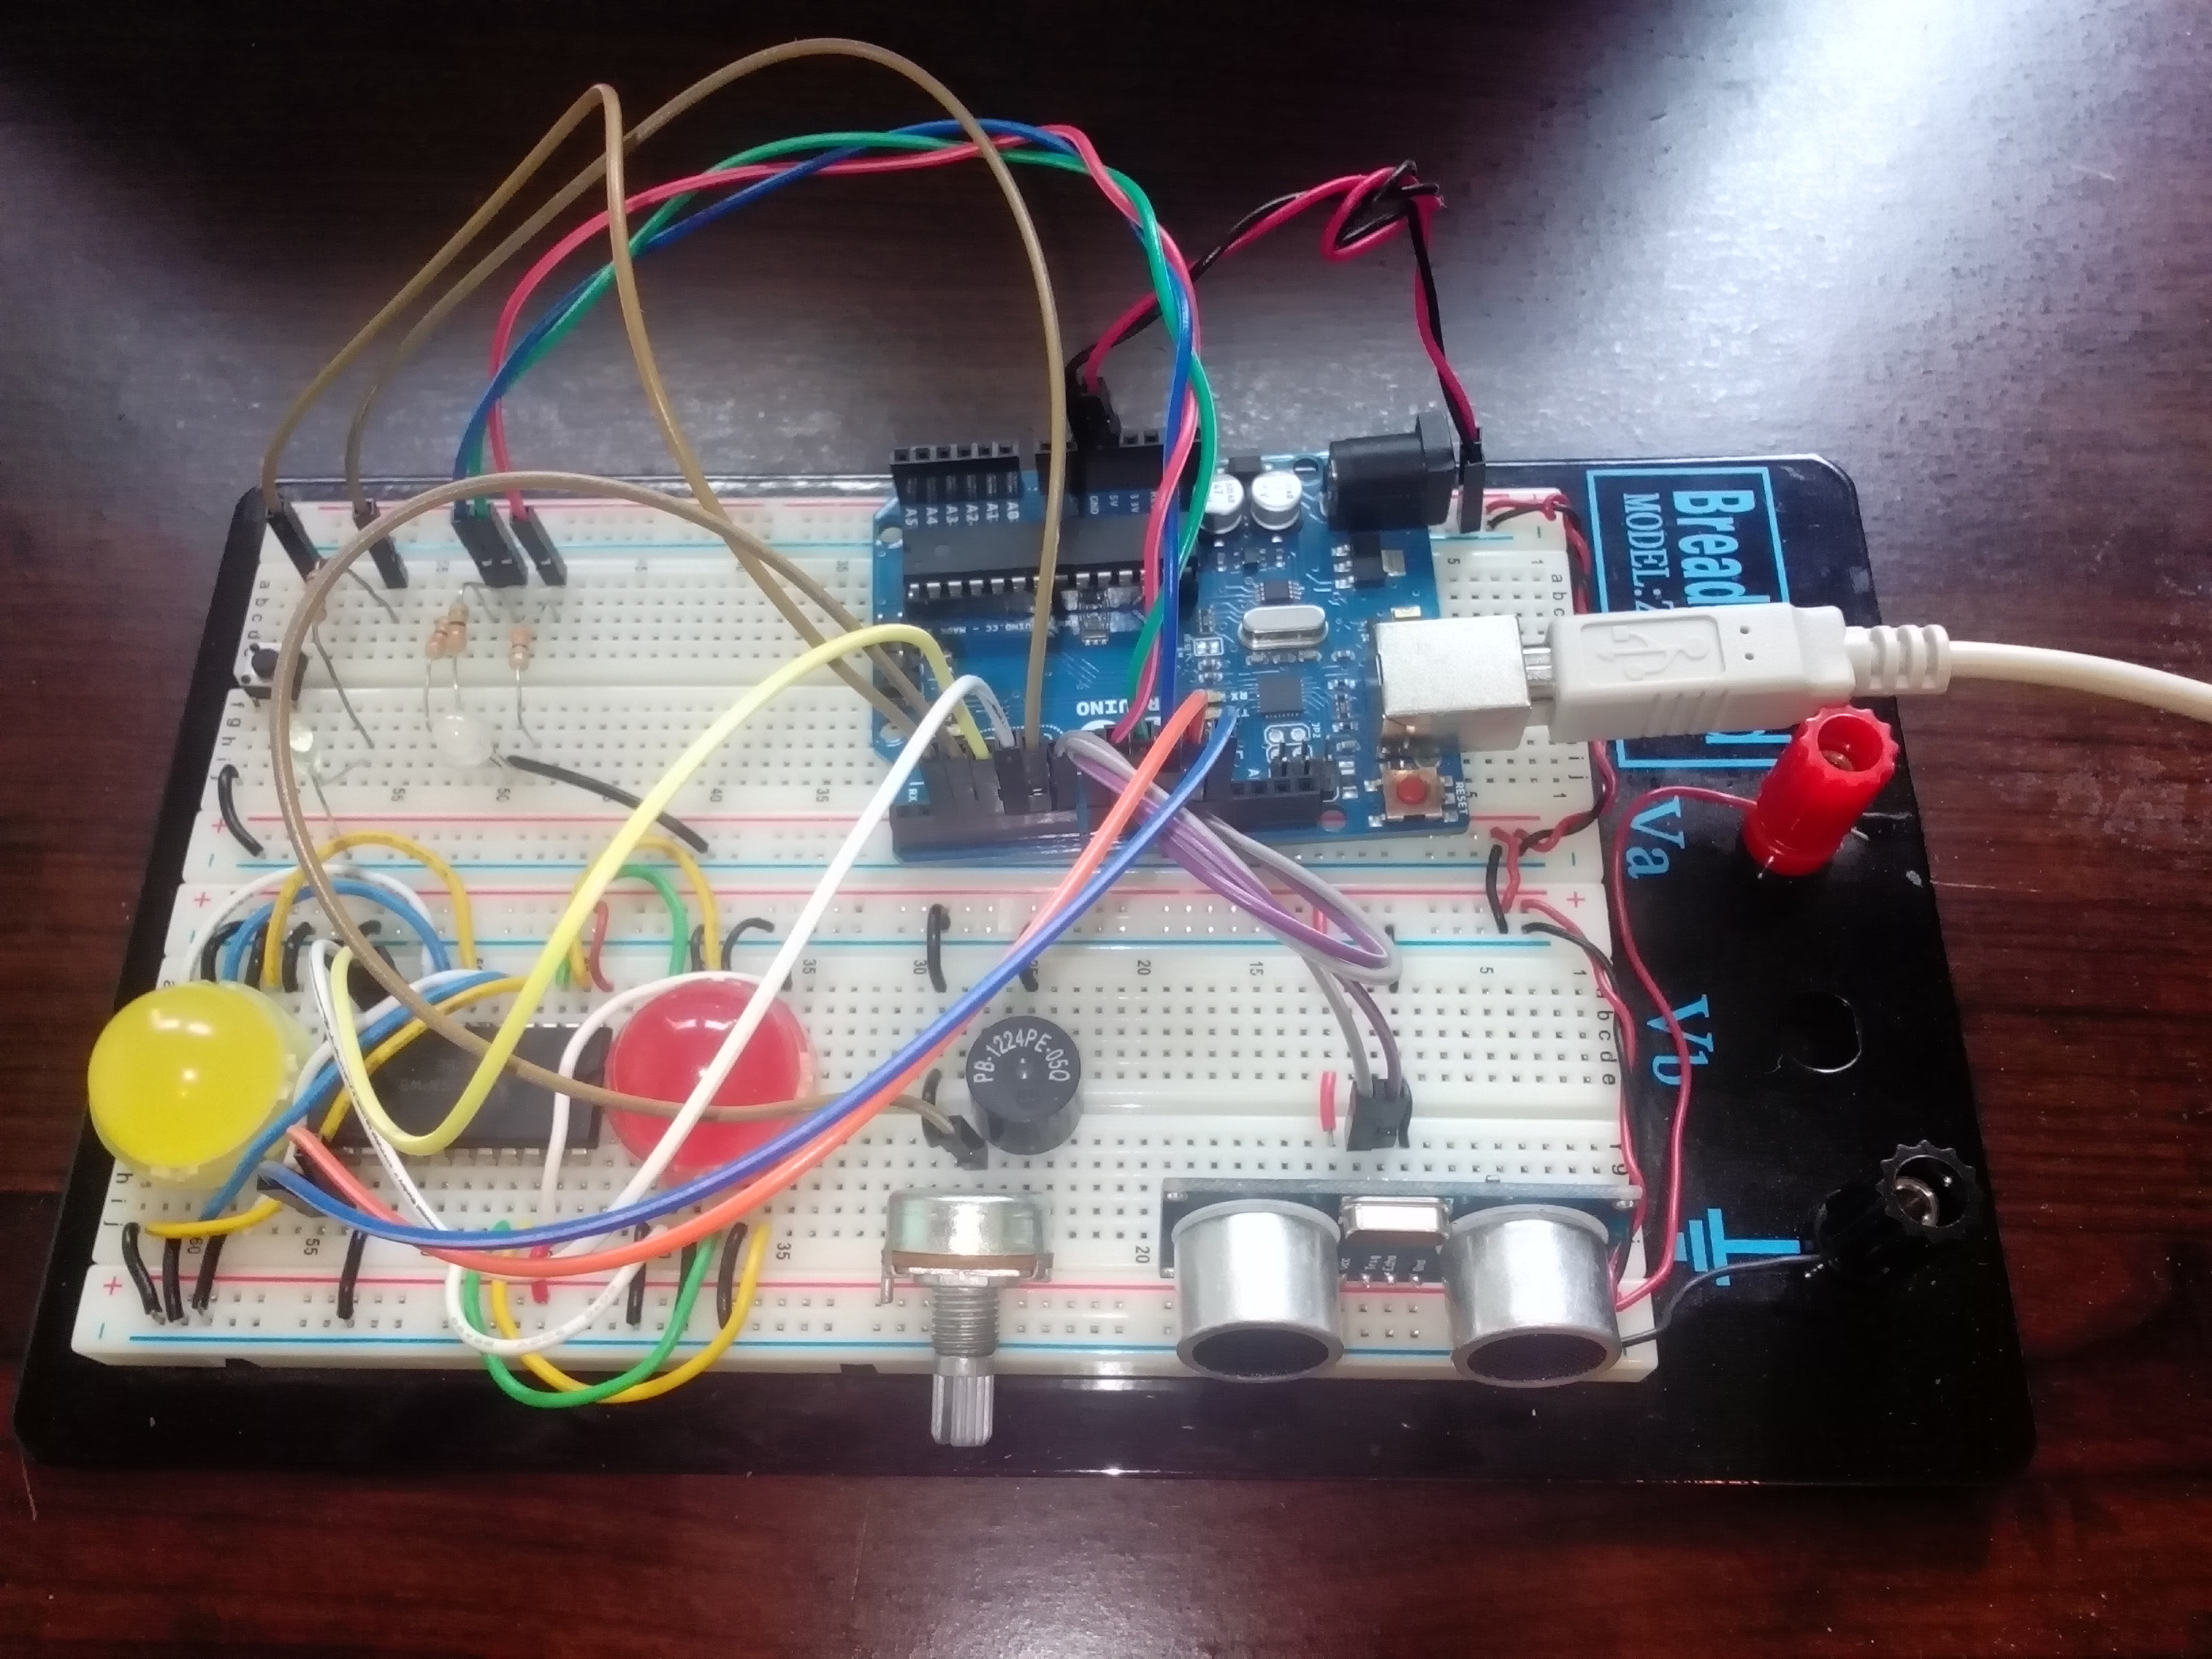
\includegraphics[scale=.08]{img/real1.jpg}
	\caption{}
	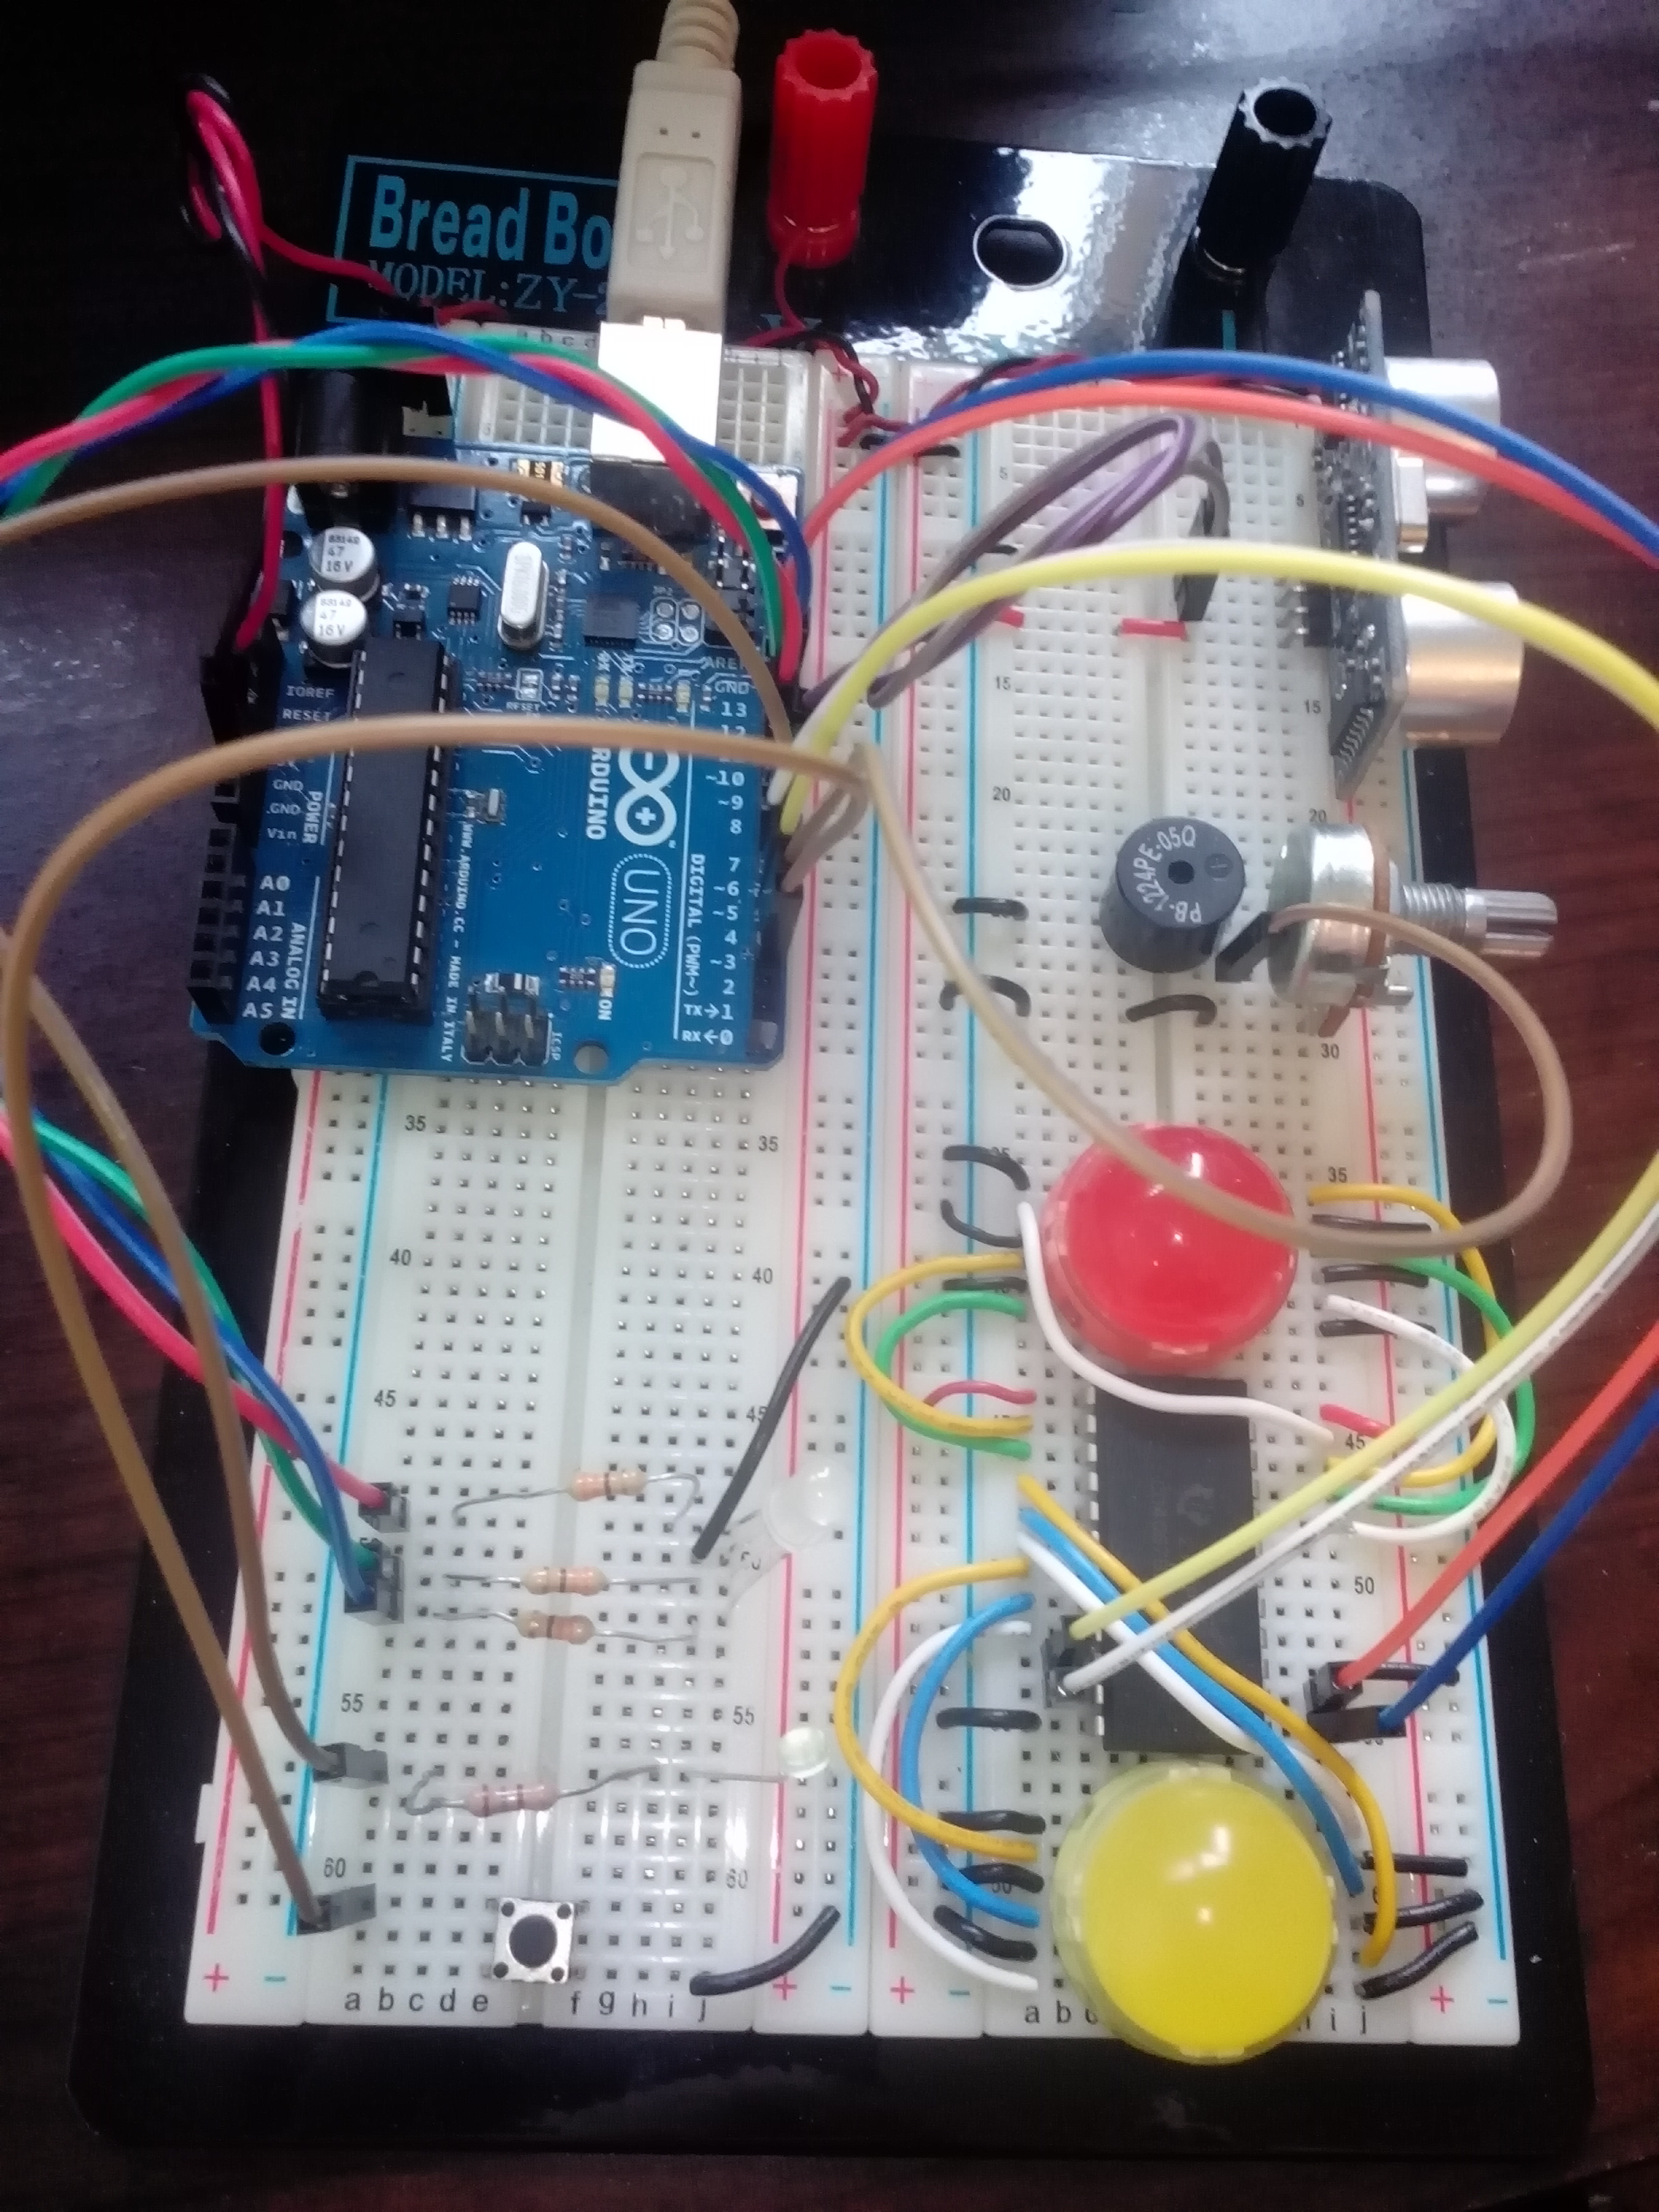
\includegraphics[scale=.08]{img/real2.jpg}
	\caption{}
\end{figure}

\section{Sketch Odroid - lato server}
\begin{figure}[!ht]
	\centering
	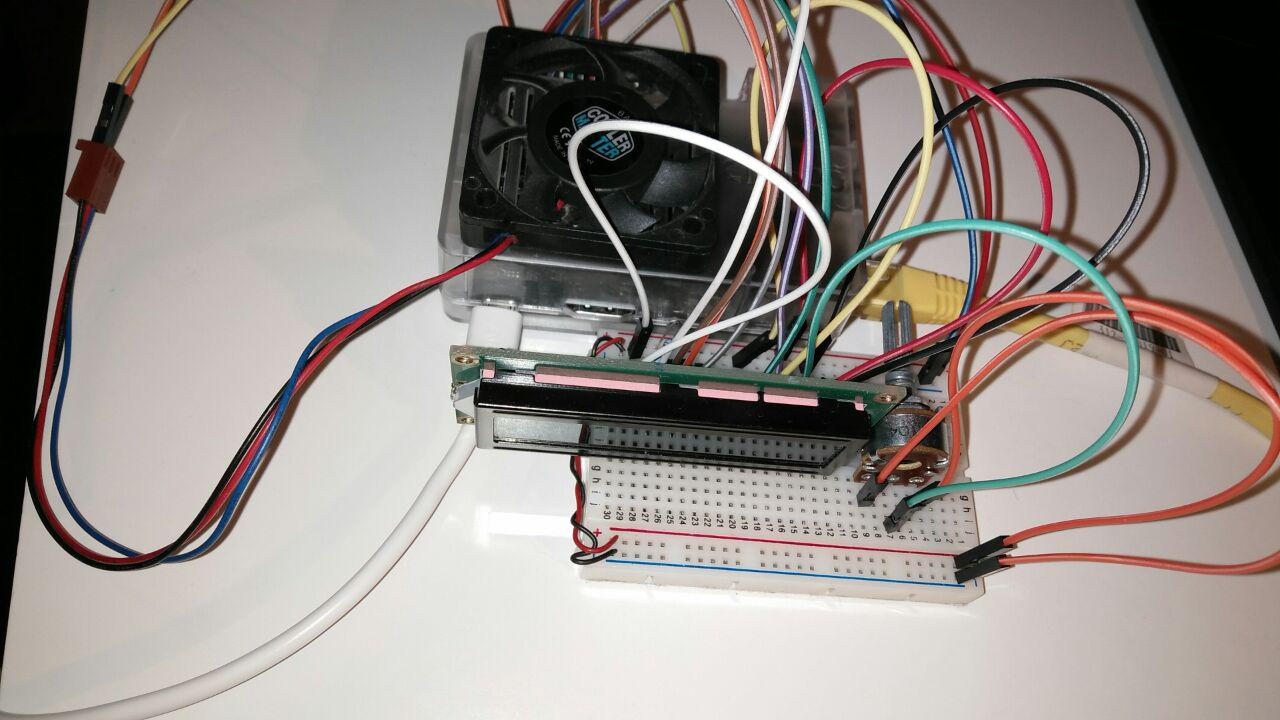
\includegraphics[scale=.3]{img/real3.jpg}
	\caption{Sketch Odroid - lato server}
\end{figure}

\begin{figure}[!ht]
	\centering
	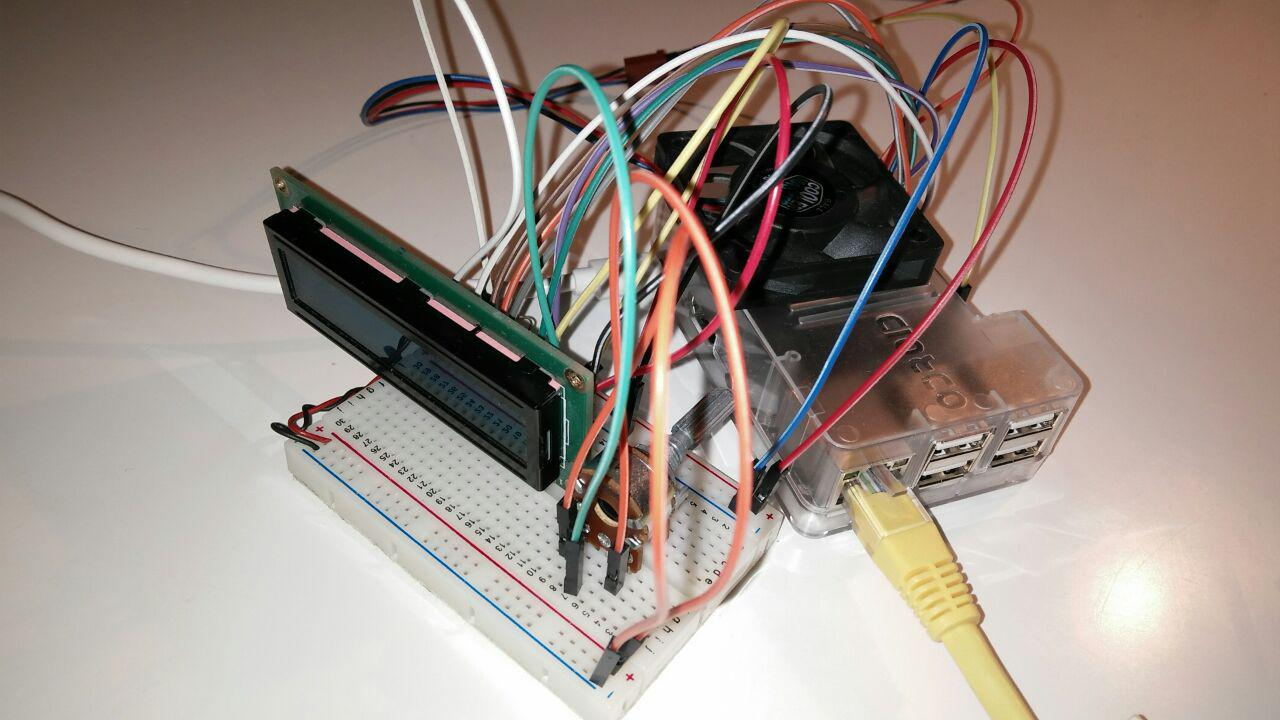
\includegraphics[scale=.3]{img/real4.jpg}
	\caption{Sketch Odroid - lato server}
\end{figure}